\documentclass[conference]{IEEEtran}
\IEEEoverridecommandlockouts
\usepackage{cite}
\usepackage{amsmath,amssymb,amsfonts}
\usepackage{algorithmic}
\usepackage{graphicx}
\usepackage{textcomp}
\usepackage{xcolor}
\usepackage{booktabs}
\usepackage{hyperref}
\usepackage{listings}
\usepackage{tikz}
\usetikzlibrary{shapes.geometric, arrows.meta, positioning, calc}

\def\BibTeX{{\rm B\kern-.05em{\sc i\kern-.025em b}\kern-.08em
    T\kern-.1667em\lower.7ex\hbox{E}\kern-.125emX}}

\lstset{
  basicstyle=\scriptsize\ttfamily,
  frame=single,
  breaklines=true,
  numbers=none,
  keywordstyle=\color{blue},
  stringstyle=\color{red},
  commentstyle=\color{green!50!black},
  showstringspaces=false
}

\begin{document}

\title{On the Duality of Basis Expansion and Coordinate-Free Representation in Geometric Computing}

\author{\IEEEauthorblockN{Intelligent Interfaces Group}}

\maketitle

\begin{abstract}
Geometric Algebra (GA), or Clifford Algebra $\operatorname{Cl}(p,q)$, provides a coordinate-free framework for physical simulation and geometric neural computing. However, implementing GA inside high-throughput computer hardware requires mapping abstract geometric elements into concrete numerical memory buffers. In this paper, we explore the duality between the coordinate-free mathematical ideal and the basis expansion representation $A = \sum_k a_k e_k$ used in modern software consoles. We analyze how basis expansions structure multivector arrays in WebAssembly/Rust memory implementations, examine the physical interpretation of grade spectral projections $\langle A \rangle_k$, and discuss how interactive lab consoles bridge the gap between low-level hardware memory layouts and coordinate-free geometric intuition.
\end{abstract}

\begin{IEEEkeywords}
Geometric Algebra, Clifford Algebra, Basis Expansion, Multivector, WebAssembly, Hardware Memory Mapping, Geometric Neural Computing
\end{IEEEkeywords}

%% ============================================================
\section{Introduction}
%% ============================================================

Geometric Algebra (GA) unifies vectors, oriented planes (bivectors), and oriented volumes (trivectors) into a single algebraic structure: the \textit{multivector}~\cite{b_hestenes}. While theoretical formulations emphasize coordinate-free operations---such as rotor rotations $R M \tilde{R}$ and wedge products $u \wedge v$---computational software systems must inevitably represent multivectors using finite numerical arrays.

At the interface of hardware execution and interactive scientific consoles, a fundamental question arises: \textit{What is the physical and structural role of the sum $A = \sum_k a_k e_k$?}

This paper examines the basis expansion of geometric elements in $\operatorname{Cl}(p,q)$, detailing its mathematical formulation, its implementation in low-level memory (e.g., Rust and WebAssembly), and its diagnostic role at the interactive lab console.

%% ============================================================
\section{Mathematical Formulations of Basis Expansion}
\label{sec:formulation}
%% ============================================================

\subsection{Grade-1 Vector Expansion}
In an $n$-dimensional vector space $\mathbb{R}^n$ equipped with an orthonormal basis $\{e_1, e_2, \dots, e_n\}$, any grade-1 vector $A \in \mathbb{R}^n$ is expressed as a linear combination of basis vectors:
\begin{equation}
    A = \sum_{k=1}^n a_k e_k = a_1 e_1 + a_2 e_2 + \dots + a_n e_n
    \label{eq:vector_expansion}
\end{equation}
where $a_k \in \mathbb{R}$ represents the scalar coordinate along the orthogonal basis direction $e_k$.

\subsection{Homogeneous \texorpdfstring{$k$}{k}-Blade Expansion}
Extending beyond vectors, higher-grade geometric elements (such as bivectors and trivectors) are formed via the antisymmetric wedge product $\wedge$. A homogeneous $k$-vector is expanded over the basis $k$-blades $E_K = e_{i_1} \wedge e_{i_2} \wedge \dots \wedge e_{i_k}$ for ordered multi-indices $K = (i_1 < i_2 < \dots < i_k)$:
\begin{equation}
    A^{(k)} = \sum_{|K|=k} a_K E_K
    \label{eq:blade_expansion}
\end{equation}
For example, in $\mathbb{R}^3$, a bivector $B$ ($k=2$) is expanded over the three canonical oriented basis planes $\{e_{12}, e_{23}, e_{31}\}$:
\begin{equation}
    B = \gamma_{12} e_{12} + \gamma_{23} e_{23} + \gamma_{31} e_{31}
\end{equation}

\subsection{General Multivector Grade Decomposition}
In the full Clifford algebra $\operatorname{Cl}(p,q)$, the algebra space is $2^n$-dimensional. Any arbitrary multivector $M$ decomposes uniquely into a sum of its homogeneous grade projections $\langle M \rangle_k$:
\begin{equation}
    M = \sum_{k=0}^n \langle M \rangle_k = \underbrace{\langle M \rangle_0}_{\text{scalar } \alpha} + \underbrace{\langle M \rangle_1}_{\text{vector } \beta} + \underbrace{\langle M \rangle_2}_{\text{bivector } \gamma} + \underbrace{\langle M \rangle_3}_{\text{trivector } \delta}
    \label{eq:grade_decomp}
\end{equation}

In 3D Euclidean space $\operatorname{Cl}(3,0)$, this yields an 8-dimensional space generated by the basis blades:
\begin{equation}
    \{ 1,\; e_1,\; e_2,\; e_3,\; e_{12},\; e_{23},\; e_{31},\; e_{123} \}
\end{equation}

%% ============================================================
\section{Hardware and Memory Mapping}
\label{sec:hardware}
%% ============================================================

While mathematicians manipulate coordinate-free expressions, computer processors operate on linear memory buffers. The basis expansion provides the bridge between geometric semantics and SIMD/cache memory architectures.

\subsection{Flat Memory Buffers in Rust and WebAssembly}
In the Sensensble Geometry platform, the $\operatorname{Cl}(3,0)$ multivector engine (\texttt{engine/src/lib.rs}) represents the general multivector $M$ as a contiguous 8-element floating-point array:
\begin{equation}
    \text{\texttt{data: [f64; 8]}} = [s,\; e_1,\; e_2,\; e_3,\; e_{12},\; e_{23},\; e_{31},\; e_{123}]
    \label{eq:array_layout}
\end{equation}

This flat memory layout offers significant performance advantages:
\begin{enumerate}
    \item \textbf{Cache Coalescing:} Storing coefficients contiguously minimizes CPU cache misses during geometric product computations.
    \item \textbf{Zero-Copy WebAssembly Interop:} The flat array layout maps directly to WebAssembly linear memory, allowing JavaScript and WebGPU to dereference multivector buffers without marshalling overhead.
    \item \textbf{gRPC Serialization:} In the distributed backend, state vectors are transmitted over gRPC as `repeated float` payloads in Protocol Buffer messages (`geometry.proto`).
\end{enumerate}

%% ============================================================
\section{The Console Perspective: Grade Spectral Analysis}
\label{sec:console}
%% ============================================================

At an interactive scientific console, the basis expansion $\sum_k a_k E_k$ serves as a \textit{grade spectrum display}---analogous to a Fourier spectrum in signal processing or an oscilloscope in electronics.

\begin{figure}[htbp]
\centering
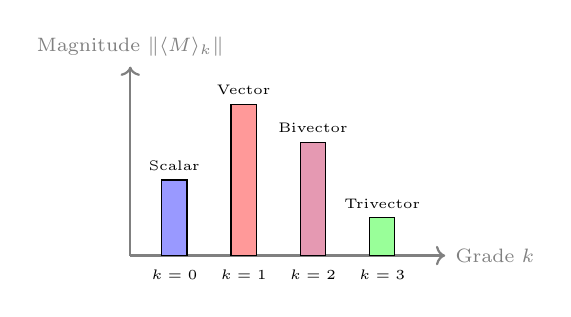
\begin{tikzpicture}[
    scale=0.8,
    bar/.style={rectangle, draw, fill=blue!30, width=0.6cm},
    axis/.style={->, thick, gray}
]
  % Axes
  \draw[axis] (0,0) -- (5,0) node[right, font=\scriptsize] {Grade $k$};
  \draw[axis] (0,0) -- (0,3) node[above, font=\scriptsize] {Magnitude $\| \langle M \rangle_k \|$};

  % Grade bars
  \draw[fill=blue!40] (0.5,0) rectangle (0.9, 1.2) node[above, font=\tiny] at (0.7, 1.2) {Scalar};
  \draw[fill=red!40] (1.6,0) rectangle (2.0, 2.4) node[above, font=\tiny] at (1.8, 2.4) {Vector};
  \draw[fill=purple!40] (2.7,0) rectangle (3.1, 1.8) node[above, font=\tiny] at (2.9, 1.8) {Bivector};
  \draw[fill=green!40] (3.8,0) rectangle (4.2, 0.6) node[above, font=\tiny] at (4.0, 0.6) {Trivector};

  \node[font=\tiny] at (0.7, -0.3) {$k=0$};
  \node[font=\tiny] at (1.8, -0.3) {$k=1$};
  \node[font=\tiny] at (2.9, -0.3) {$k=2$};
  \node[font=\tiny] at (4.0, -0.3) {$k=3$};
\end{tikzpicture}
\caption{Conceptual grade spectral analysis display at an interactive lab console, showing the distribution of geometric energy across multivector grades.}
\label{fig:spectrum}
\end{figure}

When a physical system or neural network evolves, inspecting the coefficients $a_K$ reveals the structural distribution of physical quantities:
\begin{itemize}
    \item \textbf{Grade 0 (Scalar):} Invariant mass, scalar charge, or thermodynamic energy.
    \item \textbf{Grade 1 (Vector):} Linear velocity, electric field, or directional force.
    \item \textbf{Grade 2 (Bivector):} Angular momentum, magnetic flux, or rotational vorticity.
    \item \textbf{Grade 3 (Trivector):} Volume element, helicity, or pseudoscalar chirality.
\end{itemize}

Thus, while the user authors coordinate-free equations (e.g., $R v \tilde{R}$), the console uses the basis expansion to visualize how energy transitions between grades during dynamic interaction.

%% ============================================================
\section{Conclusion}
%% ============================================================

The basis expansion $A = \sum_k a_k E_k$ is the essential link between the coordinate-free theory of Geometric Algebra and its implementation in hardware and software. By structuring multivectors as contiguous arrays in WebAssembly and gRPC, platforms like Sensensble Geometry achieve native execution speeds while preserving intuitive, grade-decomposed visual feedback at the interactive lab console.

\begin{thebibliography}{00}
\bibitem{b_hestenes} D.~Hestenes and G.~Sobczyk, \emph{Clifford Algebra to Geometric Calculus: A Unified Language for Mathematics and Physics}. Dordrecht: Reidel, 1984.
\bibitem{b_dorst} L.~Dorst, D.~Fontijne, and S.~Mann, \emph{Geometric Algebra for Computer Science}. San Francisco: Morgan Kaufmann, 2007.
\bibitem{b_ruhe} D.~Ruhe, J.~Brandstetter, and P.~Forr\'{e}, ``Clifford Group Equivariant Neural Networks,'' in \emph{Proc. NeurIPS}, 2023.
\end{thebibliography}

\end{document}
